% !TeX program = pdflatex
%
% post.tex -- a one-page, readable A4 double-column article layout example.
%
% The production pipeline is scripts/gen_a4_latex.py + scripts/gen_a4_latex.tex
% (generic, so it reads like a toolbox). If you just want to see what a "post"
% looks like, read THIS file: it needs no scripts, only `pdflatex`, and stays
% on a single page. The figure below is pulled straight from the repo root:
% assets/Edward John Poynter_Pea Blossoms, 1890.jpg
%
% NOTE: the real template typesets with MonaspiceNe NFM + Sarasa Mono SC (CJK)
% and therefore runs under xelatex/lualatex. Uncomment the fontspec lines and
% compile with xelatex to switch.

\documentclass[twocolumn]{article}

%% Page: A4, narrow margins
\usepackage[a4paper, margin=1.4cm]{geometry}

\usepackage{graphicx}   % images
\usepackage{caption}    % figure captions
\usepackage{microtype}  % microtypography / justified text
\usepackage{xcolor}     % color accents

%% Real fonts (requires xelatex/lualatex):
% \usepackage{fontspec}
% \usepackage{xeCJK}
% \setmainfont{MonaspiceNe NFM}
% \setCJKmainfont{Sarasa Mono SC}

\usepackage{duckuments} % dummy-text generator (lorem-like, but ducks)

% Compact, minimal feel
\setlength{\columnsep}{1.2em}
\setlength{\parindent}{1.5em}

\title{\textbf{The Offshoring of Thought and Memory}\thanks{dummy title}}
\author{Someone\thanks{dummy author}}
\date{}

\begin{document}
\maketitle
\vspace{-2.5em}

\section*{Introduction}
\blindduck

\blindduck

\section{What belongs where}
\blindduck

% Inline (non-floating) figure: keeps the one-page layout deterministic.
\begin{center}
\begin{minipage}{0.9\linewidth}
  \centering
  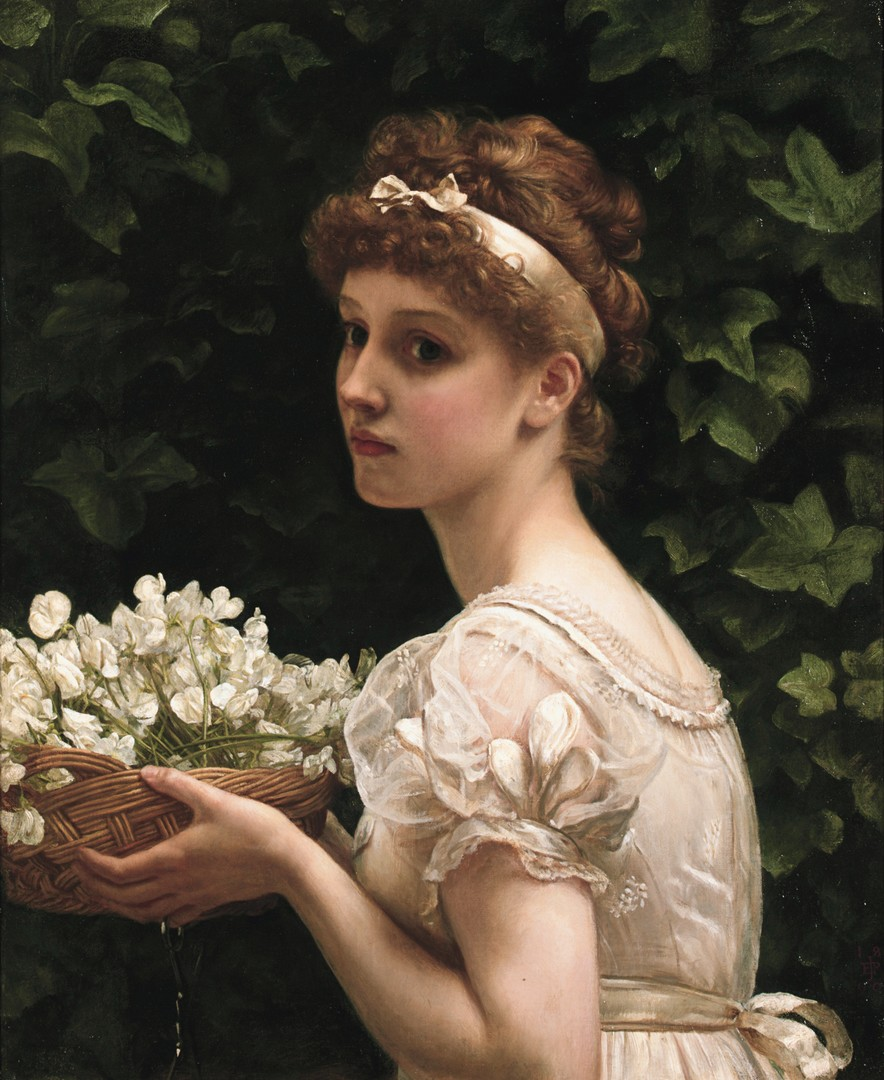
\includegraphics[width=\linewidth]{../assets/Edward John Poynter_Pea Blossoms, 1890.jpg}
  \captionof{figure}{A caption block is narrowed, centered as a block, yet its
  text stays left-aligned (90\% column width).}
\end{minipage}
\end{center}

\blindduck

\section{Memory is cheap, attention is not}
\blindduck

\end{document}
